\documentclass{beamer}

% Font selection
\usepackage{palatino}

% Beamer template
\usetheme{Antibes}
%\usetheme{Berlin}

\usepackage[scale=1.2]{ccicons}

\usepackage[utf8]{inputenc}
\usepackage[T1]{fontenc}
\usepackage[spanish]{babel}

\usepackage{tabularx}
\usepackage{multicol}
\usepackage{graphicx}
\usepackage[final]{pdfpages}

\usepackage{listings}

\lstset{
  language=C++,
  columns=flexible,
  identifierstyle=\itshape,
%
  belowcaptionskip=1\baselineskip,
  breaklines=true,
  xleftmargin=\parindent,
  language=C++,
  showstringspaces=false,
  basicstyle=\tiny,
  keywordstyle=\bfseries\color{green!40!black},
  commentstyle=\itshape\color{purple!40!black},
  identifierstyle=\color{blue},
  stringstyle=\color{brown},
  columns=flexible,
%  inputenconding=utf8,
  extendedchars=true,
%
  morekeywords=[1]{constexpr,nullptr,alignof,alignas,decltype},
  literate={%
    {¿}{{?`}}1
    {¡}{{!`}}1
    {á}{{\'a}}1
    {é}{{\'e}}1
    {í}{{\'i}}1
    {ó}{{\'o}}1
    {ú}{{\'u}}1
    {ñ}{{\~n}}1
}
}

\newcommand{\cppkey}[1]{%
{\color{green!40!black}\texttt{#1}}%
}

\newcommand{\cppid}[1]{%
{\color{blue}\texttt{#1}}%
}

\lstdefinestyle{terminal}{
  language=bash,
  basicstyle=\scriptsize\ttfamily,
  numbersep=3pt,
  frame=tb,
  columns=fullflexible,
  backgroundcolor=\color{yellow!20},
  literate=%
    {¿}{{?`}}1
    {¡}{{!`}}1
    {á}{{\'a}}1
    {é}{{\'e}}1
    {í}{{\'i}}1
    {ó}{{\'o}}1
    {ú}{{\'u}}1
    {ñ}{{\~n}}1
}


\usepackage{listings}

\lstdefinestyle{terminal}{
  language=bash,
  basicstyle=\scriptsize\ttfamily,
  numbersep=3pt,
  frame=tb,
  columns=fullflexible,
  backgroundcolor=\color{yellow!20},
  literate=%
    {¿}{{?`}}1
    {¡}{{!`}}1
    {á}{{\'a}}1
    {é}{{\'e}}1
    {í}{{\'i}}1
    {ó}{{\'o}}1
    {ú}{{\'u}}1
    {ñ}{{\~n}}1
}

\lstdefinestyle{termoutput}{
  basicstyle=\scriptsize\ttfamily,
  frame=tb,
  backgroundcolor=\color{blue!20},
  keywordstyle=\color{black},
  commentstyle=\color{black},
  identifierstyle=\color{black},
  stringstyle=\color{black},
}


\lstset{
  language=[ISO]C++,
  basicstyle=\scriptsize,
  morekeywords=[1]{constexpr,nullptr,alignof,alignas,decltype,noexcept,override,final},
}


\renewcommand{\cppkey}[1]{%
{\color{green!40!black}\textbf{#1}}%
}

\renewcommand{\cppid}[1]{%
{\color{blue}\textbf{#1}}%
}


\usepackage{tikz}
\usetikzlibrary{positioning}
\usetikzlibrary{arrows}
\usetikzlibrary{mindmap}

\usepackage{pgfplots}
\pgfplotsset{compat=1.5}


\newcommand{\textgood}[1]{%
{\color{blue}\textbf{#1}}%
}

\newcommand{\textbad}[1]{%
{\color{red}\textbf{#1}}%
}

\newcommand{\textemph}[1]{%
{\color{green!40!black}\textbf{#1}}%
}

\newcommand{\textenum}[1]{%
{\color{blue!60!black}\textbf{#1}}%
}

\newcommand{\textmark}[1]{%
{\color{orange!70!black}\textbf{#1}}%
}




% Footline in every slide
\setbeamertemplate{footline}{
  \leavevmode%
  \hbox{\begin{beamercolorbox}[wd=\paperwidth,ht=2.5ex,dp=1.125ex,leftskip=.3cm,rightskip=.3cm]{author in head/foot}%
    \usebeamerfont{author in head/foot}\ccbyncndeu 
     \quad -- \quad J. Daniel Garcia 
     -- ARCOS@UC3M (\textbf{\url{josedaniel.garcia@uc3m.es}}) 
     -- Twitter: \textbf{\url{@jdgarciauc3m}}
    \hfill
    \insertframenumber/\inserttotalframenumber
  \end{beamercolorbox}}%
  \vskip0pt%
}

% Logo in every slide
\addtobeamertemplate{headline}{}
{% 
\begin{tikzpicture}[remember picture,overlay]
\node[anchor=north east] at (current page.north east) {
\includegraphics[height=0.7cm]{logos/arcos_t.png}};
\end{tikzpicture}
}

\tikzset{
  invisible/.style={opacity=0},
  visible on/.style={alt=#1{}{invisible}},
  alt/.code args={<#1>#2#3}{%
    \alt<#1>{\pgfkeysalso{#2}}{\pgfkeysalso{#3}} % \pgfkeysalso doesn't change the path
  },
}

%Portada
\title{Matemáticas y Lenguaje C++}
\subtitle{¿Quién ayuda a quién?}
\author{J. Daniel Garcia}
\institute{Grupo ARCOS\\Universidad Carlos III de Madrid}
\date{Febrero 2019}

\begin{document}

\begin{frame}
\titlepage
\end{frame}

\AtBeginSection[]
{
  \begin{frame}<*>
    \setbeamertemplate{section in toc shaded}[default][50]
    \setbeamertemplate{subsection in toc shaded}[default][50]
    \tableofcontents[currentsection,hideallsubsections]
  \end{frame}
}

\AtBeginSubsection[]
{
  \begin{frame}<beamer>
    \setbeamertemplate{subsection in toc shaded}[default][50]
    \tableofcontents[sectionstyle=show/hide,subsectionstyle=show/shaded/hide]
  \end{frame}
}

\begin{frame}{Aviso}

\begin{tabularx}{.98\textwidth}{lX}
\ccLogo & Esta obra está bajo una Licencia Creative Commons Atribución-NoComercial-SinDerivar 4.0 Internacional.\\

\ccAttribution & 
Debes dar crédito en la obra en la forma especificada por el autor o licenciante.\\

\ccNonCommercialEU &
El licenciante permite copiar, distribuir y comunicar públicamente la obra. A
cambio, esta obra no puede ser utilizada con fines comerciales — a menos que se
obtenga el permiso expreso del licenciante.
\\

\ccNoDerivatives &
El licenciante permite copiar, distribuir, transmitir y comunicar públicamente
solamente copias inalteradas de la obra -- no obras derivadas basadas en ella.
\\

\end{tabularx}

\end{frame}

\begin{frame}{ARCOS@uc3m}
\begin{itemize}
  \item \textbf{ARCOS}: Investigación aplicada.
    \begin{itemize}
      \item {\color{blue}{Líneas}}: 
        HPC,
        Big data,
        Sistemas ciberfísicos,
        \textmark{Modelos de programación para la mejora de aplicaciones}.
    \end{itemize} 
  \vfill
  \item \textbf{Mejora de aplicaciones}:
    \begin{itemize}
      \item \textmark{REPARA}: Reengineering and Enabling Performance and poweR of Applications.
            Comisión Europea (FP7). 2013--2016.
      \item \textmark{RePhrase}: REfactoring Parallel Heterogeneous Resource Aware Applications.
            Comisión Europea (H2020). 2015--2018.
      \item \textmark{ASPIDE}: Exascale programIng models for extreme data processing.
            Comisión Europea (H2020). 2018--2020.
    \end{itemize} 
  \vfill
  \item \textbf{Normalización}:
    \begin{itemize}
      \item \textgood{ISO/IEC JTC/SC22/WG21}. ISO C++ standards committe.
        \begin{itemize}
          \item C++11, C++14, C++17, C++20, \ldots
        \end{itemize}
    \end{itemize}
\end{itemize}
\end{frame}

\section{El lenguaje C++}

\begin{frame}{¿Qué es C++?}
\begin{center}
\begin{tikzpicture}[small mindmap,
    concept color=blue,
    level 1 concept/.append style={font=\tiny,level distance=2.3cm},
    level 2 concept/.append style={font=\tiny,level distance=1.7cm},
    level 3 concept/.append style={font=\tiny},
    every node/.append style={scale=0.9},
    text=white,
    ]
  \node [concept, font=\small] {C++}
    child [grow=25, visible on=<1->] {node[concept] {Es C con ...}}
    child [grow=340, visible on=<2->] {node[concept, visible on=<2->] {Demasiado \ldots}
      child [grow=40, visible on=<3->]{node[concept] {difícil}}
      child [grow=0, visible on=<4->]{node[concept] {bajo nivel}}
      child [grow=320, visible on=<5->]{node[concept] {alto nivel}}
    }
    child [grow=90,visible on=<6->] {node[concept] {Programación}
      child [grow=20,visible on=<7->]{node[concept] {Orientada a objetos}
        child [grow=10]{node[concept] {Clases}}
        child [grow=330]{node[concept] {Jerarquías de clases}}
      }
      child [grow=150,visible on=<8->] {node[concept] {Genérica}
        child [grow=180] {node[concept] {Metapro\-gramción}}
      }
      child [grow=200,visible on=<9->]{node[concept] {Multi\-paradigma}}
    }
    child [grow=180, level distance=2.25cm,visible on=<10->] {node[concept] {Problemas}
      child [grow=200, visible on=<11->] {node[concept] {Buffer overflow}}
      child [grow=150,visible on=<11->] {node[concept] {Goteos de memoria}}
    }
    child [grow=220, visible on=<12->] {node[concept] {Un cajón de sastre}}

  ;
\end{tikzpicture}
\end{center}
\end{frame}

\begin{frame}{¿De donde viene?}
\begin{itemize}
  \item \pause Influencias de alto nivel.
    \begin{itemize}
      \item Lenguajes de abstracción de propósito general.
        \begin{itemize}
          \item Simula.
        \end{itemize}
      \item Lenguajes de abstración de dominio específico.
        \begin{itemize}
          \item FORTRAN, COBOL.
        \end{itemize}
    \end{itemize}
  \item \pause Influencias de bajo nivel.
    \begin{itemize}
      \item Correspondencia directa con el hardware.
        \begin{itemize}
          \item Ensamblador.
        \end{itemize}
      \item Abstracción mínima del hardware.
        \begin{itemize}
          \item BCPL.
          \item C.
        \end{itemize}
    \end{itemize}
  \item \pause Influencias sobre otros lenguajes.
    \begin{itemize}
      \item Java.
      \item C\#.
      \item C (C11).
    \end{itemize}
\end{itemize}
\end{frame}

\begin{frame}{¿Qué es C++11/14/17?}
\begin{itemize}
  \item \pause ISO/IEC 14882:2011, 14882:2014, 14882:2017.
  \item \pause Son la siguientes versiones de C++03.
  \item \pause \emph{``Un lenguaje de programación de abstracciones ligeras''} (B. Stroustroup).
  \item \pause C++11.
    \begin{itemize}
      \item Contiene muchas mejoras sobre C++98/03.
      \item Tiene muchos elementos de compatibilidad.
        \begin{itemize}
          \item La raíz histórica de algunos llega hasta 1972.
        \end{itemize}
      \item Evolucionar un lenguaje con miles de millones de línea de código es
      distinto que diseñar un nuevo lenguaje de programación.
    \end{itemize}
  \item \pause Si alguien dice que tiene un lenguaje de programación perfecto:
    \begin{itemize}
      \item Es na\"{i}ve.
      \item Es un vendedor.
    \end{itemize}
\end{itemize}
\end{frame}


\begin{frame}[t]{El comité ISO C++}
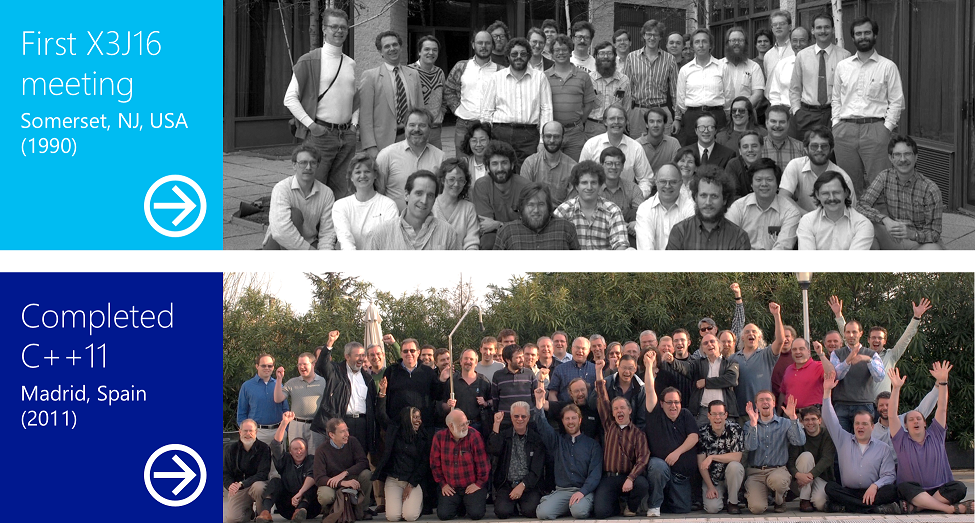
\includegraphics[width=\textwidth]{img/wg21-1990-2011.png}
\end{frame}

\begin{frame}[t]{C++14}
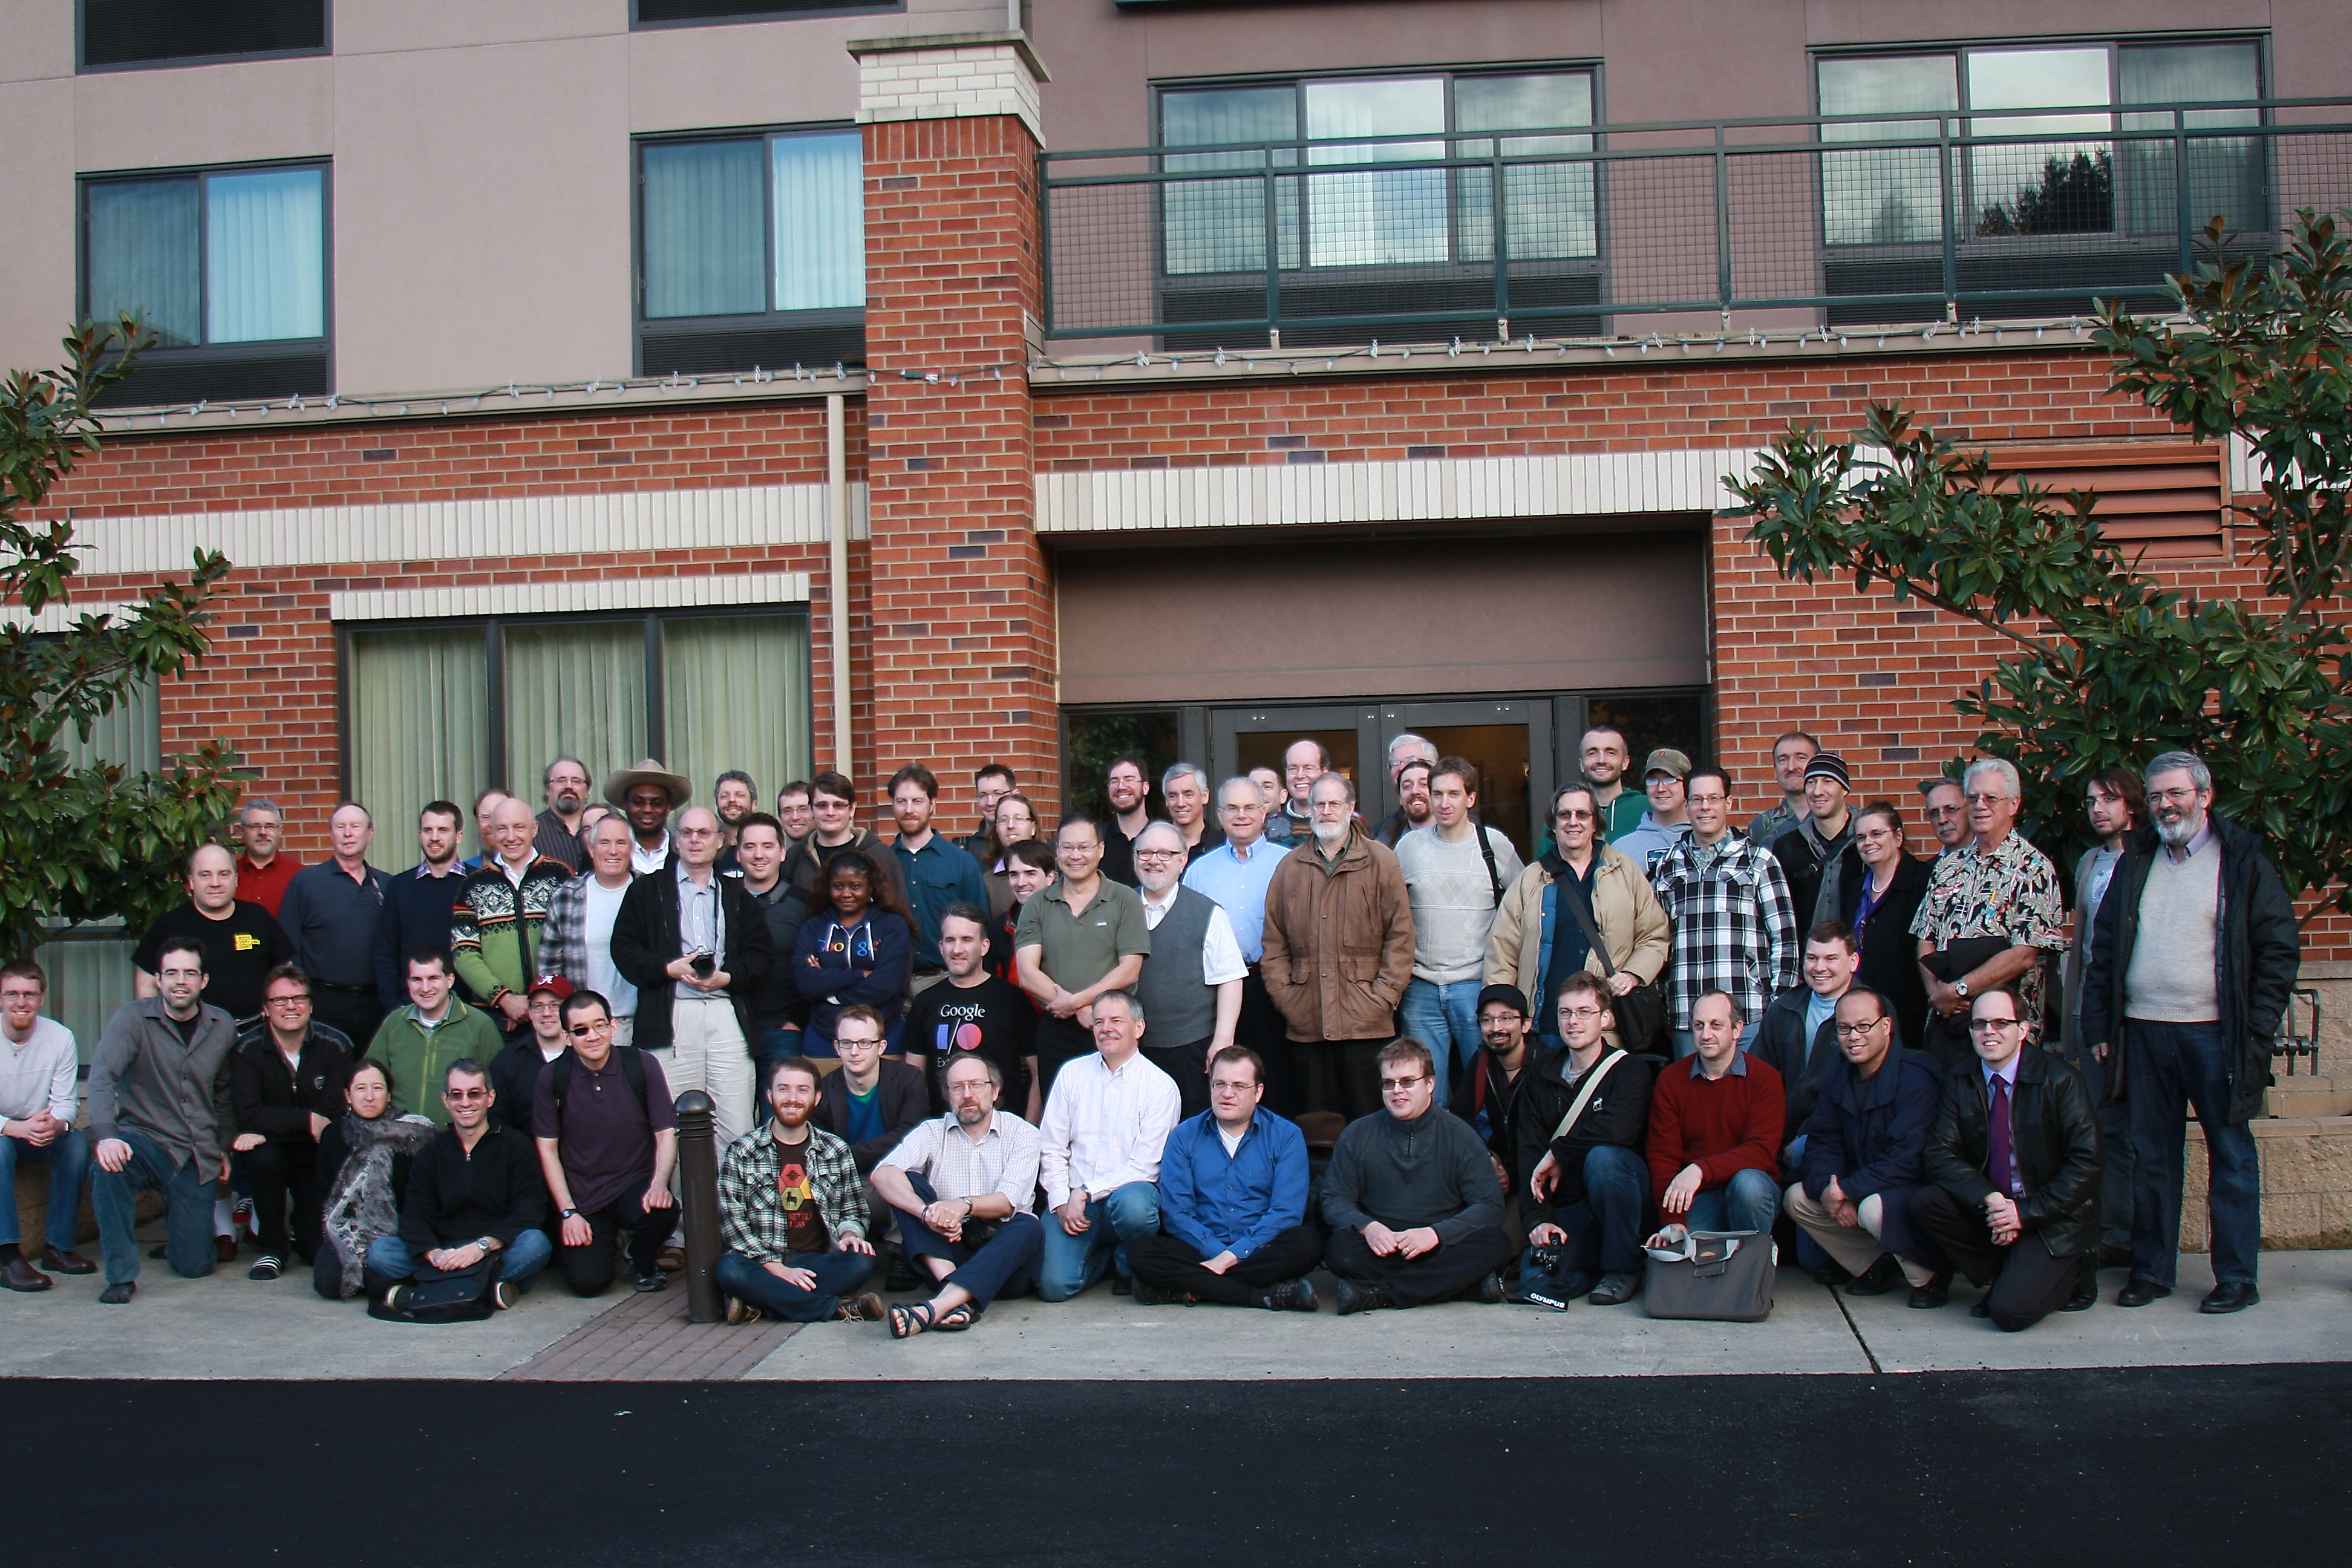
\includegraphics[width=\textwidth]{img/cpp-14.jpg}
\end{frame}

\begin{frame}[t]{C++17}
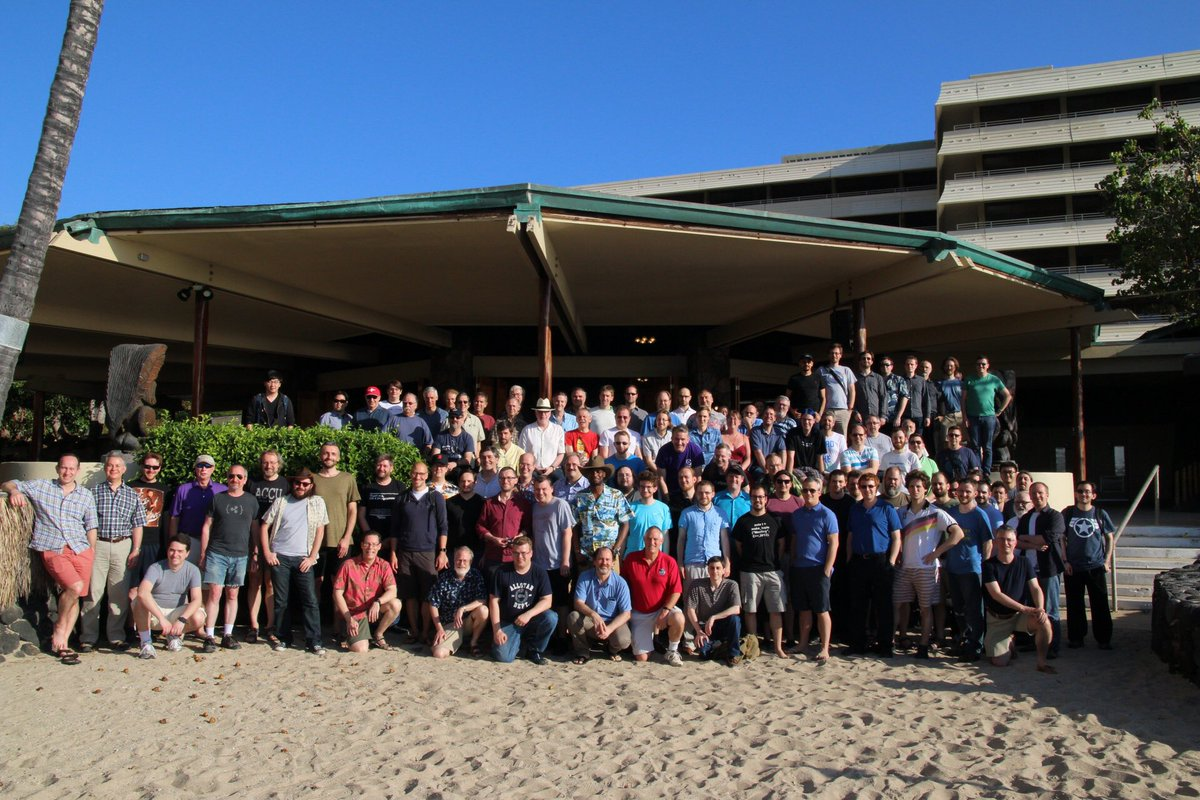
\includegraphics[width=\textwidth]{img/cpp-17.jpg}
\end{frame}

\begin{frame}[t,fragile]{¿Qué pinta tiene?}
\begin{lstlisting}
int main() {
}
\end{lstlisting}
\end{frame}

\begin{frame}[t]{Una breve historia}
\begin{itemize}
  \item 1998: \textgood{C++98} $\rightarrow$ \textmark{ISO/IEC 14882:1998}.

  \vfill\pause
  \item 2003: \textgood{C++03} $\rightarrow$ \textmark{ISO/IEC 14882:2003}.
    \begin{itemize}
      \item \textemph{Technical Corrigendum}.
    \end{itemize}

  \vfill\pause
  \item 2005: \textgood{C++ TR1} $\rightarrow$ \textmark{ISO/IEC TR 19768}.
    \begin{itemize}
      \item \textemph{C++ Library Extensions}.
    \end{itemize}

  \vfill\pause
  \item 2011: \textgood{C++11} $\rightarrow$ \textmark{ISO/IEC 14882:2011}.

  \vfill\pause
  \item 2014: \textgood{C++14} $\rightarrow$ \textmark{ISO/IEC 14882:2014}. 

  \vfill\pause
  \item 2017: \textgood{C++17} $\rightarrow$ \textmark{ISO/IEC 14882:2017}.

  \vfill\pause
  \item 2020: \textgood{C++20} $\rightarrow$ \textbad{ISO/IEC 14882:????}.
\end{itemize}
\end{frame}

\begin{frame}{C++ timeline}
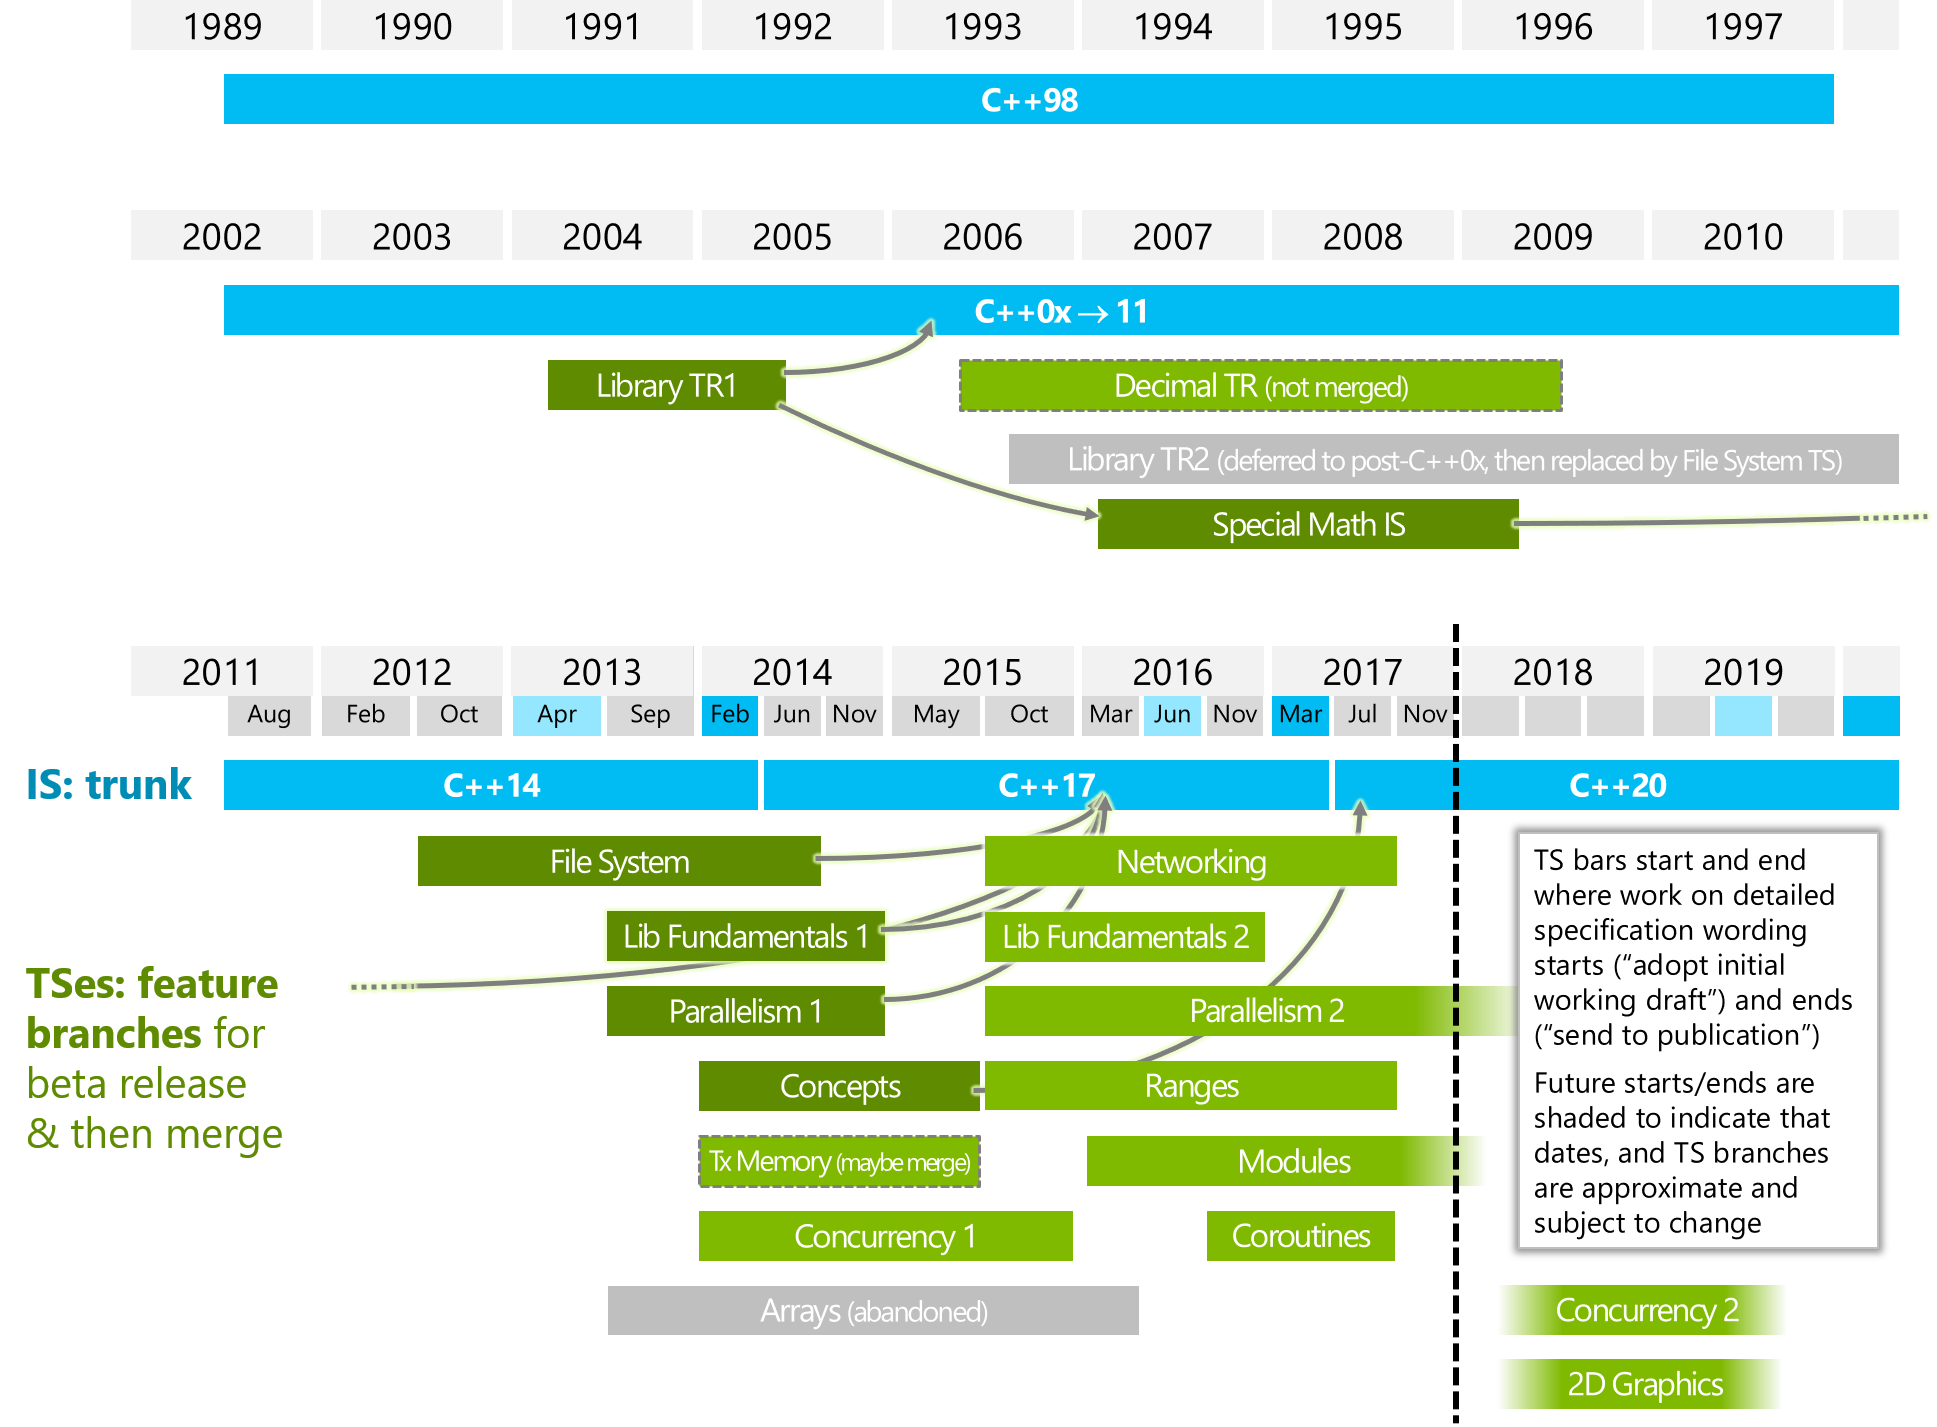
\includegraphics[height=.8\textheight]{img/wg21-timeline.png}
\end{frame}

\begin{frame}[t]{Principios de diseño}
\begin{itemize}
  \item \vfill\pause  Mantener \textmark{compatibilidad} hacia atrás.
  \item \vfill\pause  Mejor \textmark{extender} la biblioteca que el lenguaje.
  \item \vfill\pause  Facilitar el \textmark{diseño} de sistemas y bibliotecas (en vez de dominios concretos).
  \item \vfill\pause  Mejorar la \textmark{seguridad de tipos}.
  \item \vfill\pause  Mejorar el \textmark{rendimiento} y la \textmark{interacción con el hardware}.
  \item \vfill\pause  Principio de \textmark{zero-overhead}.
  \item \vfill\pause  Hacer C++ \textmark{más fácil} de enseñar y aprender.
\end{itemize}
\end{frame}

\begin{frame}{El comité C++}
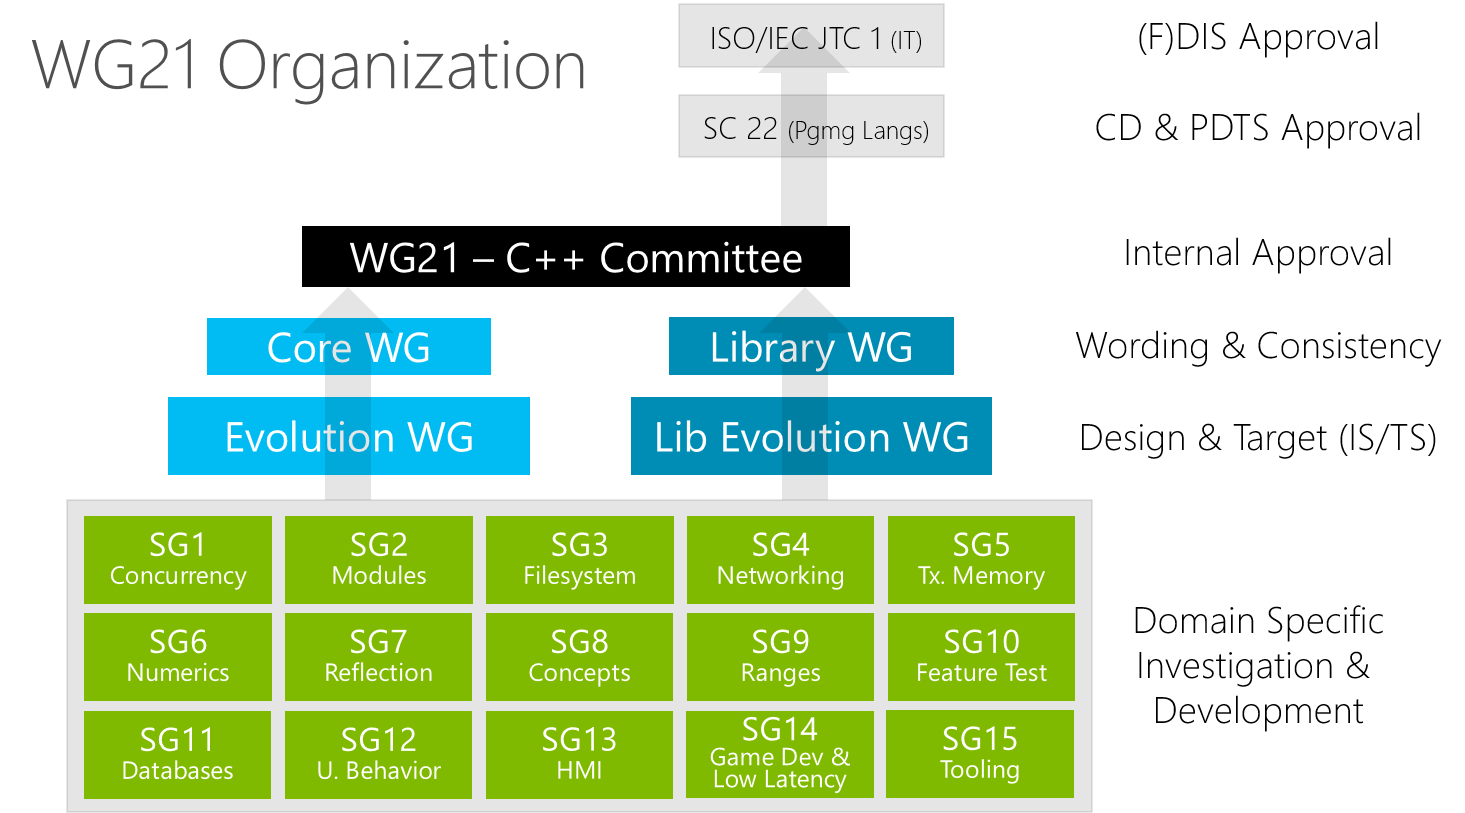
\includegraphics[width=\textwidth]{img/wg21-structure.png}
\end{frame}



\section{Programación genérica}

\subsection{Templates}

\begin{frame}[t]{Polimorfismo}
\begin{itemize}
  \item \textmark{Polimorfismo}: Permite que valores de distintos tipos
        lleven a cabo una misma operación de distinta forma.
    \begin{itemize}
      \item Permite poder expresar componentes software de forma genérica.
    \end{itemize}

  \vfill\pause
  \item \textmark{Tipos de polimorfismo}:
    \begin{itemize}
      \item \textgood{Polimorfismo dinámico} $\Rightarrow$ 
            \textmark{Prog. orientada a objetos}.
      \item \textgood{Polimorfismo estático} $\Rightarrow$
            \textmark{Prog. genérica}.
    \end{itemize}

  \vfill\pause
  \item \textmark{Importante}: C++ soporta los dos tipos de polimorfismo.
\end{itemize}
\end{frame}

\begin{frame}[t]{Ventajas del polimorfismo estático}
\begin{itemize}
  \item \textgood{Rendimiento}: Código con menos sobrecoste en tiempo de ejecución
    \begin{itemize}
      \item Se toman más decisiones en tiempo de compilación.
      \item Más amigable para el optimizador del compilador.
      \item Código más predecible $\Rightarrow$ Tiempo real duro.
      \item Útil en computación numérica.
    \end{itemize}

  \vfill\pause
  \item \textgood{Flexibilidad}: Integración de componentes software diseñados
        de forma separada.
    \begin{itemize}
      \item Posibilidad de construir tipos genéricos complejos.
      \item Es la arquitectura de la propia biblioteca estándar de C++.
    \end{itemize}
\end{itemize}
\end{frame}

\begin{frame}[t,fragile]{Programación genérica}
\begin{itemize}
  \item Mecanismo para alcanzar polimorfismo estático.
\begin{lstlisting}
template <typename T>
T square(T x) {
  return x*x;
}
\end{lstlisting}

  \pause\vfill
  \item \textmark{Objetivo}: Construir componentes que puedan operar con
        distintos tipos de datos.

  \pause\vfill
  \item Los tipos deben cumplir requisitos sintácticos y semánticos.
    \begin{itemize}
      \item Los requisitos se deducen de forma implícita.
    \end{itemize}
\end{itemize}
\end{frame}

\begin{frame}[t,fragile]{Plantillas de función}
\begin{block}{Funciones genéricas}
\begin{lstlisting}
template <typename T>
T square(T x) {
  return x * x;
}
\end{lstlisting}
\end{block}

\vfill\pause

\begin{block}{Utilización}
\begin{lstlisting}[escapechar=@]
void f() {
  std::cout << square(2.0) << "\n";    // square<double>@\pause@
  std::cout << square(1.5f) << "\n";   // square<float>@\pause@
  std::cout << square(3) << "\n";      // square<int>@\pause@
  std::cout << square("hola") << "\n"; // No válido
}
\end{lstlisting}
\end{block}

\end{frame}

\begin{frame}[t,fragile]{Tipos genéricos}
\vspace{-1em}
\begin{block}{Un tipo para coordenadas}
\vspace{-0.25em}
\begin{lstlisting}
template <typename T, int D>
class coordenada {
public:
  //...
  double distancia(coordenada q) const;
private:
  T v[D];
}
\end{lstlisting}
\vspace{-1em}
\end{block}

\vfill\pause
\begin{block}{Uso}
\vspace{-0.25em}
\begin{lstlisting}[escapechar=@]
void f() {
  coordenada<double,3> a,b;
  //...
  std::cout << a.distancia(b) << "\n";@\pause@
  //...
  coordenada<string,2> z; // ???
}
\end{lstlisting}
\end{block}
\end{frame}

\subsection{Contenedores, iteradores, algoritmos}

\begin{frame}[t]{STL: Standard Template Library}
\begin{itemize}
  \item Alex Stepanov.
    \begin{itemize}
      \item Abstracción a partir de algoritmos concretos y eficientes.
      \item Obtención de algoritmos que se pueden usar con distintas represetaciones
            de datos.
      \item Una de las claves del éxito de C++.
    \end{itemize}

  \vfill\pause
  \item Elementos de STL:
    \begin{itemize}
      \item Diversidad de contenedores.
      \item Iteradores sobre contenederes.
      \item Algoritmos independientes de contenedores expresados en
            términos de iteradores.
    \end{itemize}
\end{itemize}
\end{frame}

\begin{frame}[t,fragile]{¿Qué es un contenedor?}
\begin{itemize}
  \item Un \textgood{contenedor} es una estructura que puede
        \textmark{almacenar valores}.
    \begin{itemize}
      \item En STL los contenedores son homogéneos.
    \end{itemize}

  \vfill\pause
  \item Tipos principales de contenedores:
    \begin{itemize}
      \item \textmark{Contenedores de secuencia}: Almacenan una secuencia de valores.
      \item \textmark{Contenedores asociativos}: Almacenan pares \emph{clave-valor}.
    \end{itemize}
\end{itemize}
\end{frame}

\begin{frame}[t,fragile]{Contenedores de secuencia}
\begin{itemize}
  \item Almacenan una secuencia de valores de un determinando tipo.
  \item Pueden permitir el acceso mediante operaciones propias o
        a través de iteradores.
  \item Varios compromisos: \cppid{vector}, \cppid{list}, \cppid{deque}, \cppid{forward\_list}.
\end{itemize}
\begin{block}{Reduciendo un vector}
\begin{lstlisting}
double suma(std::vector<double> & v) {
  double r = 0.0;
  for (size_t i=0; i<v.size(); ++i) {
    r += v[i];
  }
  return r;
}
\end{lstlisting}
\end{block}
\end{frame}

\begin{frame}[t,fragile]{Iteradores}
\begin{itemize}
  \item Un \textgood{iterador} es un valor que permite recorrer los elementos
        de un contenedor.
    \begin{itemize}
      \item Cada contenedor tiene un tipo de iterador asociado.
    \end{itemize}

  \vfill\pause
  \item Operaciones mínimas:
    \begin{itemize}
      \item Acceder al objeto apuntado (\cppid{*i}).
      \item Avanzar al siguiente elemento (\cppid{++i}).
      \item Comparar si apuntan a la misma posición (\cppid{i!=j}).
    \end{itemize}

  \vfill\pause
  \item Posiciones especiales:
    \begin{itemize}
      \item \textgood{Inicio}: Primera posición del contenedor.
      \item \textgood{Fin}: Siguiente a la última posición del contenedor.
    \end{itemize}
  \vfill
  \item \textmark{Observación}: Cualquier subsecuencia se puede representar
        como un intervalo semiabierto \cppid{[i,j)}.
\end{itemize}
\end{frame}

\begin{frame}[t,fragile]{Uso de iteradores}
\begin{block}{Reducción de un vector}
\begin{lstlisting}[escapechar=@]
double suma1(std::vector<double> & v) {
  double r = 0.0;
  for (typename std::vector<double>::iterator i = v.begin(); i!=v.end(); ++i) {
    r += *i;
  }
  return r;
}
@\pause@
double suma2(std::vector<double> & v) {
  double r = 0.0;
  for (auto i = v.begin(); i!=v.end(); ++i) {
    r += *i;
  }
  return r;
}
\end{lstlisting}
\end{block}
\end{frame}

\begin{frame}[t,fragile]{Algoritmos}
\begin{itemize}
  \item Un \textgood{algoritmo} sobre una secuencia de datos se puede
        definir en términos de los iteradores que definen la secuencia.
    \begin{itemize}
      \item Esto independiza los algoritmos de las estructuras de datos concretas.
      \item Hace los algoritmos válidos para estructuras de datos que 
            todavía no existen.
    \end{itemize}
\end{itemize}
\vfill\pause
\begin{block}{Reducción de un vector}
\begin{lstlisting}
double suma(const std::vector<double> & v) {
  return std::reduce(v.begin(), v.end());
}
\end{lstlisting}
\end{block}
\end{frame}

\subsection{Expresiones lambda}

\begin{frame}[t,fragile]{Lambdas}
\begin{itemize}
  \item Inspiradas en cálculo lambda y programación funcional.
  \item Permiten definir funciones de orden superior.
\end{itemize}
\vfill\pause
\begin{block}{Ordenación en valor absoluto}
\begin{lstlisting}
void ordena_abs(std::vector<double> & v) {
  std::sort(v.begin(), v.end(),
    [](double x, double y) { return std::abs(x) < std::abs(y); }
  );
}
\end{lstlisting}
\end{block}
\end{frame}

%\subsection{Rangos}


\begin{frame}[t]{Para saber más}
\begin{itemize}
  \item \textmark{Elements of Programming}.
  Alexander Stepanov, Paul McJones.
  Addison-Wesley, 2009.

  \vfill

  \item \textmark{From Mathematics to Generic Programming}.
  Alexander Stepanov.
  Addison-Wesley, 2014.

  \vfill

  \item \textmark{The C++ Standard Library -- A Tutorial and Reference, 2nd Edition}.
  Nicolai Josutis.
  Addison-Wesley, 2012.
\end{itemize}
\end{frame}

\section{El coste de la abstracción}

\begin{frame}[t]{Todo el mundo sabe que...}
\begin{itemize}
  \pause
  \item C++ es más lento que C.
    \begin{itemize}
      \item Debe serlo puesto que es de más alto nivel.
    \end{itemize}

  \vfill\pause
  \item La abstracción siempre tiene un precio en tiempo de ejecución.
    \begin{itemize}
      \item Así que no hay nada como el código de bajo nivel.
      \item Si puede ser en ensamblador.
    \end{itemize}

  \vfill\pause
  \item El mejor rendimiento se obtiene con optimizaciones de bajo nivel.
    \begin{itemize}
      \item Cuanto más pegado al hardware mejor.
    \end{itemize}

  \vfill\pause
  \item Cada enfoque de resolución de un problema necesita una versión distinta
        del código.
    \begin{itemize}
      \item No va a ser lo mismo una versión secuencial que una con OpenMP.
    \end{itemize}
\end{itemize}
\end{frame}

\begin{frame}[t]{Caso práctico: Fludianimate}
\begin{itemize}
  \item Parte del benchmark PARSEC.
    \begin{itemize}
      \item \url{http://parsec.cs.princeton.edu}
      \item Originalmente desarrollado por Intel.
      \item Versiones en simple y doble precisión.
      \item Versiones secuencial, PThreads, Intel TBB.
    \end{itemize}

  \vfill\pause
  \item Características:
    \begin{itemize}
      \item en su mayoría código tipo-C.
      \item Uso de preprocesador.
      \item Funciones sin paso de parámetros accediendo a globales.
      \item Pool de memoria ajustado a caché de procesador.
    \end{itemize}
  
\end{itemize}
\end{frame}

\begin{frame}{Métricas}
\begin{tabular}{|l|r|r|}
\hline
Métrica & Original & Refactorizado\\
\hline
\hline
Lines		& 1873	& 1330\\
Effective LOC 	& 1093	& 846\\
Logical LOC 	& 880	& 449 \\
\hline
Functions	& 87	& 125\\
Max Cyclomatic Complexity	& 33	& 8\\
Average Cycolomatic Complexity	& 3.39	& 1.35\\
\hline
Classes		& 6	& 16 \\
Max Cyclomatic Complexity	& 65 & 45\\
Average Cyclomatic Complexity	& 11.00 & 9.12\\
\hline
\end{tabular}
\end{frame}

\begin{frame}{Tiempo de ejecución por iteración}
\begin{tikzpicture}
\begin{semilogyaxis}[xlabel=Iterations,ylabel=Normalized Execution time (us), legend pos=south east]
\addplot table[header=false]{perf-fluid/p2000/fanimate.seq.norm.dat};
\addlegendentry{original}
\addplot table[header=false]{perf-fluid/p2000/animate.seq.norm.dat};
\addlegendentry{refactored}
\end{semilogyaxis}
\end{tikzpicture}
\end{frame}

\begin{frame}{Tiempo de ejecución por iteración (4 cores, 8 threads)}
\begin{tikzpicture}
\begin{semilogyaxis}[xlabel=Iterations,ylabel=Normalized Execution time (us), legend pos=south east]
\addplot table[header=false]{perf-fluid/p500/fanimate.tbb.8.norm.dat};
\addlegendentry{original}
\addplot table[header=false]{perf-fluid/p500/animate.tbb.8.norm.dat};
\addlegendentry{refactored}
\end{semilogyaxis}
\end{tikzpicture}
\end{frame}

\begin{frame}[t]{Para saber más}
\begin{itemize}
  \item \textmark{Improving performance and maintainability through refactoring in C++11}.
        J.D. Garcia y B. Stroustrup.
        ISO C++ Foundation, 2015.
        \url{https://isocpp.org/blog/2015/10/garcia-stroustrup-refactoring}.
\end{itemize}
\end{frame}

\section{Utilidades}

\subsection{Números complejos}

\begin{frame}[t,fragile]{Números complejos}
\begin{itemize}
  \item Definidos en la biblioteca estándar de forma paramétrica.
    \begin{itemize}
      \item Para tipo \cppid{T} $\in$ $\{ \cppid{float}, \cppid{double}, \cppid{long double} \}$
    \end{itemize}
\end{itemize}
\begin{block}{Ejemplo}
\begin{lstlisting}
void f() {
  using namespace std;
  using namespace std::complex_literals;

  complex<double> a = 2 + 3i;
  complex<double> b = 2 - 3i;
  complex<double> c = -2 + 5i;
  
  auto d = cos(a * b + c);
 
  cout << "Magnitud: " << abs(d) << ", ángulo: " << arg(d) << "\n";
}
\end{lstlisting}
\end{block}
\end{frame}

\subsection{Números aleatorios}

\begin{frame}[t]{Motores de generación}
\begin{itemize}
  \item Generadores pseudoaleatorios:
    \begin{itemize}
      \item \cppid{linear\_congruential\_engine}.
      \item \cppid{mersenne\_twister\_engine}.
      \item \cppid{subtract\_with\_carry\_engine}.
    \end{itemize}
  \pause\vfill
  \item Adaptdores de motores:
    \begin{itemize}
      \item \cppid{discard\_block\_engine}.
      \item \cppid{independent\_bits\_engine}.
      \item \cppid{shuffle\_order\_engine}.
    \end{itemize}
  \pause\vfill
  \item Generadores no deterministas:
    \begin{itemize}
      \item \cppid{randon\_device}.
    \end{itemize}
\end{itemize}
\end{frame}

\begin{frame}[t]{Motores de generación}
\begin{itemize}
  \item Generan valores enteros uniformes de algún tipo entero.
    \begin{itemize}
      \item Basado en una semilla.
      \item Distintos compromisos entre velocidad y almacenamiento.
      \item Muy genéricos
        \begin{itemize}
          \item Requiren parametrización cuidadosa.
        \end{itemize}
    \end{itemize}
  \vfill\pause
  \item Casos más comunes predefinidos:
    \begin{itemize}
      \item \cppid{minstd\_rand0}, \cppid{minstd\_rand} $\Rightarrow$ Congruencial lineal.
        \begin{itemize}
          \item Lewis, Goodman, Miller (1969).
        \end{itemize}
      \item \cppid{mt19937}, \cppid{mt19937\_64} $\Rightarrow$ Mersenne-Twister.
        \begin{itemize}
          \item Matsumoto, Nishimura (1998, 2000).
        \end{itemize}
      \item \cppid{ranlux24}, \cppid{ranlux48}.
        \begin{itemize}
          \item L\"{u}scher, James (1994).
        \end{itemize}
      \item \cppid{knuth\_b}
    \end{itemize}
\end{itemize}
\end{frame}

\begin{frame}[t]{Distribuciones}
\begin{itemize}
  \item Distribuciones uniformes.
    \begin{itemize}
      \item \cppid{uniform\_int\_distribution}, \cppid{uniform\_real\_distribution}.
    \end{itemize}
  \vfill\pause
  \item Distribuciones de Bernoulli.
    \begin{itemize}
      \item
        \cppid{bernoulli\_distribution},
        \cppid{binomial\_distribution},
        \cppid{negative\_binomial\_distribution},
        \cppid{geometric\_distribution}.
    \end{itemize}
  \vfill\pause
  \item Distribuciones de Poisson.
    \begin{itemize}
      \item
        \cppid{poisson\_distribution},
        \cppid{exponential\_distribution},
        \cppid{gamma\_distribution},
        \cppid{weibull\_distribution},
        \cppid{extreme\_value\_distribution}.
    \end{itemize}
  \vfill\pause
  \item Distribuicones normales.
    \begin{itemize}
      \item
        \cppid{normal\_distribution},
        \cppid{log\_normal\_distribution},
        \cppid{chi\_squared\_distribution},
        \cppid{cauchy\_distribution},
        \cppid{fisher\_f\_distribution},
        \cppid{student\_t\_distribution}.
    \end{itemize}
\end{itemize}
\end{frame}

\begin{frame}[t,fragile]
\begin{block}{Múltiples fuentes aleatorias}
\begin{lstlisting}
int main() {
  using namespace std;
  seed_seq seq{1,2,3,4};
  vector<uint32_t> seeds{10};
  seq.generate(sees.begin(), seeds.end());
  
  vector<mt19935_64> engines;
  for (int i=0; i<10; ++i) {
    engines.emplace_back(engines[i]);
  }

  normal_distribution dist{25.0, 1.5};
  for (int i=0; i<max; ++i) {
    for (auto & e : engines) {
      cout << "valor " << i << " , dist " << j << ":"
           << dist(e[j]) << "\n";
    }
  }
}
\end{lstlisting}
\end{block}
\end{frame}

\subsection{Funciones matemáticas especiales}

\begin{frame}[t]{Funciones matemáticas especiales}
\begin{itemize}
  \item Origen:
    \begin{itemize}
      \item \textgood{2007}: Informe técnico \textmark{ISO/IEC TR 17968:2007}.
      \item \textgood{2010}: Estándar internacional \textmark{ISO/IEC 29124:2010}.
      \item \textgood{2017}: Incorporadas a C++17 \textmark{ISO/IEC 14882:2017}.
    \end{itemize}

  \vfill\pause
  \item Funciones:
    \begin{itemize}
      \item Leguerre: Polinomio asociado, polinomio de Leguerre.
      \item Legendre: Polinomio asociado, polinomio de Legendre.
      \item Hermite: Polinomio de Hermite.
      \item Funciones elípticas: Primera, segunda y tercera integral elíptica.
        \begin{itemize}
          \item Completas e incompletas.
        \end{itemize}
      \item Funciones de Bessel: Regular, irregular, de primer orden.
        \begin{itemize}
          \item Cilíndricas y esféricas.
        \end{itemize}
      \item Integral exponencial.
      \item Otras funciones: Función beta, función z de Rieman.. 
    \end{itemize}
  
\end{itemize}
\end{frame}

\begin{frame}[t,fragile]{Ejemplo}
\begin{block}{Polinomios}
\begin{lstlisting}
int main() {
  using namespace std;

  cout << "Hermite3(10)" << hermite(3,10) << "\n";
  cout << "Legendre3(0.25)" << legendre(3,0.25) << "\n";
  cout << "Leguerre3(0.5)" << leguerre(3,0.25) << "\n";
}
\end{lstlisting}
\end{block}
\end{frame}

\subsection{Matrices numéricas}

\begin{frame}[t,fragile]{Arrays de valores}
\begin{itemize}
  \item Un \cppid{valarray<T>} es un array de valores numéricos.
    \begin{itemize}
      \item Garantiza la ausencia de ciertos tipos de \emph{aliasing}.
      \item Especialmente amigable con la vectorización.
    \end{itemize}
\end{itemize}
\pause
\begin{block}{Ejemplo}
\begin{lstlisting}
std::valarray<double> v = get_values();
std::valarray<double> w = get_values();
std::valarray<double> z = v + 4 * w;
\end{lstlisting}
\end{block}
\begin{itemize}
  \item \textbad{Nota}: Permite operaciones con slices generalizados
        multidemensionales.
\end{itemize}
\end{frame}

\begin{frame}[t]{Soporte de Álgebra lineal}
\begin{itemize}
  \item Evolución en bibliotecas de terceras partes.
  \vspace{2em}
  \item Trabajo actual hacia la estandarización de una biblioteca de álgebra lineal.
    \begin{itemize}
      \item Marco temporal: 2020--2023.
    \end{itemize}
\end{itemize}
\end{frame}

%\subsection{Álgebra lineal}


\begin{frame}[t]{Para sabrer más}
\begin{itemize}
  \item \textmark{The C++ Programming Language, 4th Edtion}.
        Bjarne Stroustrup.
        Addison-Wesley, 2013.

  \vfill
  \item ISO/IEC 29124:2010.
        \textmark{Extensions to the C++ Library to support mathematical special functions}.
        International Standard. 
        ISO.

  \vfill
  \item P1417R0: \textmark{Historical lessons for C++ linear algebra library standardization}.
        M. Hoemmen, J. Badwaik, M. Brucher, A. Iliopolos, J. Michopoulos.
        ISO/IEC JTC1/SC22/WG21 working paper, Enero, 2019.
        \url{wg21.link/p1417}.
        
        
\end{itemize}
\end{frame}

\section{Conceptos}

\begin{frame}[t]{Gran éxito de la programación genérica}
\begin{itemize}
  \item Algunas razones:
    \begin{itemize}
      \item Flexibilidad: Las plantillas son un sub-lenguaje \textmark{Turing-complete}.

      \vfill\pause
      \item Seguridad en tipos: Detección de inconsistencias en tiempo de compilación.

      \vfill\pause
      \item Mecanismos de especialización.
        \begin{itemize}
          \item Tipos irregulares.
          \item Metaprogramación genérica.
          \item Optimizaciones basadas en tipos.
        \end{itemize}

      \vfill\pause
      \item Rendimiento superior.
    \end{itemize}
\end{itemize}
\end{frame}

\begin{frame}[t]{Pero...}
\begin{itemize}
  \item También tiene grandes inconvenientes
    \begin{itemize}
      \vfill\item Sintaxis verbosa.
      \vfill\item \emph{Duck-typing}.
      \vfill\item Mensajes de error incomprensibles.
      \vfill\item Sobrecarga confusa.
      \vfill\item Problemas de organización de código.
      \vfill\item Compilación lenta.
    \end{itemize}
\end{itemize}
\end{frame}

\begin{frame}[t,fragile]
\begin{block}{Sumando de forma genérica}
\begin{lstlisting}
template <typename T>
T suma(const vector<T> & v) {
  T r{};
  for (auto i = v.begin(); i!=v.end(); ++i) {
    r+= *i;
  }
}

void f() {
  std::vector<double> v { 1.0, 2.0, 3.0 };
  std::cout << suma(v) << "\n";

  std::vector<complex<float>> w = readvalues();
  std::cout << suma(v) << "\n";

  std::vector<std::string> u {"C++", "mola"};
  std::cout << suma(u) << "\n"; // un no es un vector de números???
}
\end{lstlisting}
\end{block}
\end{frame}

\begin{frame}[t]{Tipos y conceptos}
\begin{itemize}
  \item \textgood{Tipo}:
    \begin{itemize}
      \item Especifica el conjunto de valores que puede tomar una entidad.
      \item Define el conjunto de operaciones que son aplicables a sus valores.
      \item Especifica la representación en memoria.
    \end{itemize}

  \vfill\pause
  \item \textgood{Concepto}:
    \begin{itemize}
      \item Especifica el conjunto de tipos que satisfacen el concepto.
      \item Define el conjunto de operaciones que son aplicables a sus valores.
      \item \textbad{No} especifica la representación en memoria.
    \end{itemize}
\end{itemize}
\end{frame}

\begin{frame}[t,fragile]
\begin{block}{Sumando de forma genérica}
\begin{lstlisting}
template <typename N>
  requires Number<N>
N suma(const vector<N> & v) {
  N r{};
  for (auto i = v.begin(); i!=v.end(); ++i) {
    r+= *i;
  }
}

void f() {
  std::vector<double> v { 1.0, 2.0, 3.0 };
  std::cout << suma(v) << "\n";

  std::vector<complex<float>> w = readvalues();
  std::cout << suma(v) << "\n";

  std::vector<std::string> u {"C++", "mola"};
  std::cout << suma(u) << "\n"; // un no es un vector de números???
}
\end{lstlisting}
\end{block}
\end{frame}

\begin{frame}[t,fragile]
\begin{block}{Sumando de forma genérica}
\begin{lstlisting}
template <Number N>
N suma(const vector<N> & v) {
  N r{};
  for (auto i = v.begin(); i!=v.end(); ++i) {
    r+= *i;
  }
}

void f() {
  std::vector<double> v { 1.0, 2.0, 3.0 };
  std::cout << suma(v) << "\n";

  std::vector<complex<float>> w = readvalues();
  std::cout << suma(v) << "\n";

  std::vector<std::string> u {"C++", "mola"};
  std::cout << suma(u) << "\n"; // un no es un vector de números???
}
\end{lstlisting}
\end{block}
\end{frame}

\begin{frame}[t,fragile]{Definiendo conceptos}
\begin{block}{El concepto \emph{Number}}
\begin{lstlisting}
template <typename N>
concept Number =
  requires (N x, N y) {
    { N{} };
    { N{x} };
    { x += y } -> N&;
  };
\end{lstlisting}
\end{block}
\end{frame}

\begin{frame}[t]{Para saber más}
\begin{itemize}
  \item ISO/IEC TS 19217:2015: \textmark{C++ Extensions for Concepts}.
        Technical Specification.
        ISO.

  \vfill
  \item \textmark{Concepts: The future of generic programmiing (the future is here)}.
        Bjarne Stroustrup.
        \url{https://youtu.be/PU-2ntDuF10}
\end{itemize}
\end{frame}

\section{Programación basada en contratos}

\begin{frame}[t]{Corrección frente a robustez}
\begin{itemize}
  \item En el diseño de un componente hay una tensión entre
        dos propiedades \textmark{relacionadas} y \textmark{ortogonales}:
    \begin{itemize}
      \item \textgood{robustez}.
      \item \textgood{corrección}.
    \end{itemize} 

  \vfill\pause
  \item \textgood{Robustez}: Capacidad de un componente de reaccionar
        de forma apropiada a condiciones anormales.

  \vfill\pause
  \item \textgood{Corrección}: Grado en el que un componente software
        cumple con su especificación.
\end{itemize}
\end{frame}

\begin{frame}[t]{Programación basada en contratos}
\begin{itemize}
  \item Basada originalmente en las ideas de la \textmark{lógica de Hoare}.
    \begin{itemize}
      \item Conceptos de \textgood{precondición} y \textgood{postcondición}.
    \end{itemize}
  \vfill\pause
  \item Desarrollado posteriormente por Bertrand Meyer en el lenguaje Eiffel.
  \vfill
  \item Metáfora de componentes como \textgood{cliente} y \textgood{servidor}
        que se relacionan mediante un \textmark{contrato} con 
        \textmark{obligaciones} y \textmark{beneficios}.
    \begin{itemize}
      \item\pause Las \textgood{precondiciones} son una 
          \textmark{obligación} para el \textgood{cliente} y un
          \textmark{beneficio} para el \textgood{suministrador}.
      \item\pause Las \textgood{postcondiciones} son una
          \textmark{obligación} para el \textgood{suministrador} y un
          \textgood{beneficio} para el \textmark{cliente}.
    \end{itemize}
\end{itemize}
\end{frame}

\begin{frame}[t,fragile]{Comprobaciones}
\begin{itemize}
  \item Una \textmark{comprobación} es un predicado que forma parte
        de un contrato y que se comprueba en tiempo de ejecución
        para determinar si el software tiene un defecto.
\end{itemize}
\begin{block}{Contrato para una pila}
\begin{lstlisting}
template <typename T>
class stack {
public:
  stack() [[ensures: size() == 0]];

  int size() [[ensures r: r>=0]];

  void push(const T & x)
    [[expects: !is_full()]]
    [[ensures: !is_empty()]];
  //...
}
\end{lstlisting}
\end{block}
\end{frame}

\begin{frame}[t,fragile]{Axiomas}
\begin{itemize}
  \item Un \textmark{Axioma} es un postulado que se tiene por cierto.
    \begin{itemize}
      \item Se pueden utilizar en el análisis de los programas para
            determinar inconsistencias.
      \item Se pueden utilizar durante la optimización del programa.
      \item Permiten el uso de predicados que no son \emph{idempotentes}.
    \end{itemize}
\end{itemize}
\begin{block}{Axiomas de la búsqueda binaria}
\begin{lstlisting}
template <typename Iter, typename T>
Iter busqueda_binaria(Iter primero, Iter ultimo, T value)
  [[expect axiom: se_puede_llegar(primero,ultimo)]]
  [[expect audit: esta_ordenado(primero,ultimo)]]
  [[ensures axiom res: se_puede_llegar(primero,res) &&
                       se_puede_llegar(res,ultimo)]];
\end{lstlisting}
\end{block}
\end{frame}

\begin{frame}[t]{Para saber más}
\begin{itemize}
  \item \textmark{An axiomatic basis for computer programming}.
        C.A.R. Hoare.
        Communications of the ACM, 12(1):576--580.
        1969.

  \vfill
  \item \textmark{Object Oriented Software Construction}.
        Bertrand Meyer.
        Prentice-Hall, 1997.

  \vfill
  \item P0542R5: \textmark{Support for contract based programming in C++}
        G. Dos Reis, J.D. Garcia, J. Lakos, A. Meredith, N. Myers, B. Stroustrup.
        ISO/IEC JTC1/SC22/WG21 working paper. Junio 2018.
        \url{http://wg21.link/p0542r5}.
\end{itemize}
\end{frame}

\section{Paralelismo}

\begin{frame}[t]{Programación secuencial frente a paralela}
\begin{itemize}
  \item \textmark{Programación secuencial}:
    \begin{itemize}
      \item Conjunto bien conocido de \emph{estructuras de control}
            como parte de los lenguajes de programción.
      \item Estructuras de control \emph{inherentement secuenciales}
    \end{itemize}

  \vfill\pause
  \item \textmark{Programación paralela tracional}:
    \begin{itemize}
      \item Construcciones que adaptan las estructuras de control
            secuencial al mundo paralelo (p.ej. \emph{parallel-for}).
    \end{itemize}

  \vfill\pause
  \item Pero \ldots
    \begin{itemize}
      \item ¿Y si pudiesemos tener estructuras que fuesen a la vez
            secuneciales y paralelas?
    \end{itemize}
\end{itemize}
\end{frame}

\begin{frame}[t]{Diseño de software}

\begin{quote}
There are two ways of constructing a software design:\\ 
\vspace{1em}
\pause
One way is\\
\pause
to make it \textgood{so simple} that there are \textmark{obviously no deficiencies},\\
\pause
\vspace{.5em}
and the other way is\\
\pause
to make it \textgood{so complicated} that there are \textmark{no obvious deficiencies}.\\ 
\vspace{1em}
\pause
The \textmark{first method} is \textbad{far more difficult}. 
\end{quote}
\hfill C.A.R Hoare
\end{frame}

\begin{frame}[t,fragile]{Ejemplo: Transformando una secuencia}
\begin{itemize}
  \item Dada una secuencia de \cppid{frame}s, generar una 
        nueva secuencia en escala de grises.
\begin{lstlisting}
struct frame { /*...*/ };
frame togray(const frame & f);
\end{lstlisting}
\end{itemize}
\begin{center}
\input{frame-map.tkz}
\end{center}
\end{frame}

\begin{frame}[t,fragile]{Transformando una secuencia}
\begin{block}{Bucle tradicional explícito}
\lstinputlisting[firstline=6,lastline=17]{ej/src/togray/loop.cpp}
\end{block}
\end{frame}

\begin{frame}[t,fragile]{Transformando una secuencia}
\begin{block}{Al estilo STL}
\lstinputlisting[firstline=6,lastline=17]{ej/src/togray/stl-transform.cpp}
\end{block}
\end{frame}

\begin{frame}[t,fragile]{Transforming a sequence}
\begin{block}{Al estilo STL paralelo (C++17)}
\lstinputlisting[firstline=6,lastline=17]{ej/src/togray/pstl-transform.cpp}
\end{block}
\end{frame}

\begin{frame}[t]{Más allá del estándar: GrPPI}
\begin{itemize}
  \item \textgood{GrPPI}: Generic Reusable Parallel Pattern Interface.
    \begin{itemize}
      \vfill\item
      Separación de \textmark{código de aplicación} y \textmark{modelo de ejecución}.

      \vfill\item
      Composición mediante \textmark{patrones de diseño} paralelos.

      \vfill\item
      \textmark{Modelos soportados}:
        \begin{itemize}
        \item Secuencial.
        \item ISO C++ Threads.
        \item Open MP.
        \item Intel TBB.
        \item FastFlow.
        \item Dinámico.
        \end{itemize}
    \end{itemize}
\end{itemize}
\end{frame}

\begin{frame}[t]{Patrones de paralelismo}
\begin{itemize}
  \item \textgood{Patrones de datos}: Expresan cómputo sobre un conjunto de datos.
    \begin{itemize}
      \item \textmark{map}, \textmark{reduce}, \textmark{map/reduce}, \textmark{stencil}.
    \end{itemize}

  \vfill\pause
  \item \textgood{Patrones de tareas}: Expresan composiciones de tareas.
    \begin{itemize}
      \item \textmark{divide/conquer}.
    \end{itemize}

  \vfill\pause
  \item \textgood{Patrones de flujo}: Expresan cómputo sobre un flujo de datos 
        (posiblemente sin límite).
    \begin{itemize}
      \item \textmark{pipeline}.
      \item Specialized stages: \textmark{farm}, \textmark{filter}, 
            \textmark{reduction}, \textmark{iteration}.
    \end{itemize}
\end{itemize}
\end{frame}

\begin{frame}[t,fragile]{Ejemplo: Procesamiento de imagen}
\begin{block}{Mejora de imágenes}
\begin{lstlisting}
void procesa(std::istream & is, std::ostream & os) {
  grppi::parallel_omp_execution ex;

  grppi::pipeline(ex,
    [&]() -> optional<frame> {
      auto f = read_frame();
      if (is) return f;
      else return {};
    },
    grppi::discard([](const frame & f) { return f.low_quality();}),
    [](const frame & f) { return filter(f); },
    [](const frame & f) { return togray(f); },
    [&](const frame & f) { write_frame(os,f); }
  );
}
\end{lstlisting}
\end{block}
\end{frame}

\begin{frame}[t]{Resonancia Magnética Cerebral}
\begin{columns}
\column{.7\textwidth}
\begin{itemize}
  \item Método no intrusivo para acceder a la anatomía interna.
  \item Grandes cantidades de datos generadas.
  \item Aplicaciones en neurociencias.
    \begin{itemize}
      \item Desorden bipolar.
      \item Paranoia.
      \item Esquizofrenia.
    \end{itemize}
\end{itemize}

\column{.3\textwidth}
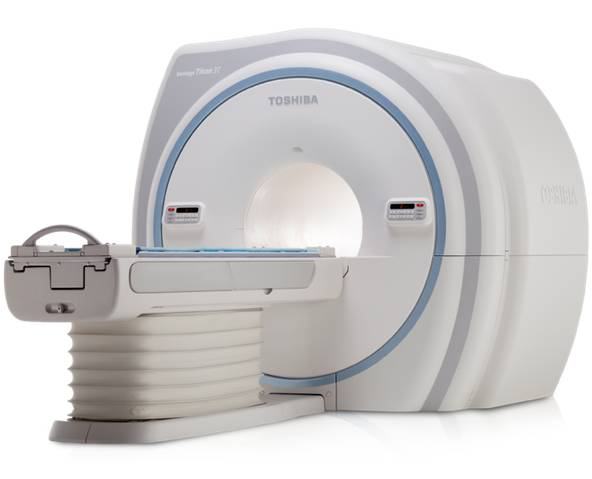
\includegraphics[width=\textwidth]{img/mri-scanner.jpg}
\end{columns}

\vspace{2em}
\begin{itemize}
  \item Identificación de fibras y conectividad entre áreas del cerebro.
\end{itemize}

\end{frame}

\begin{frame}[t]{Fibras}
\begin{center}
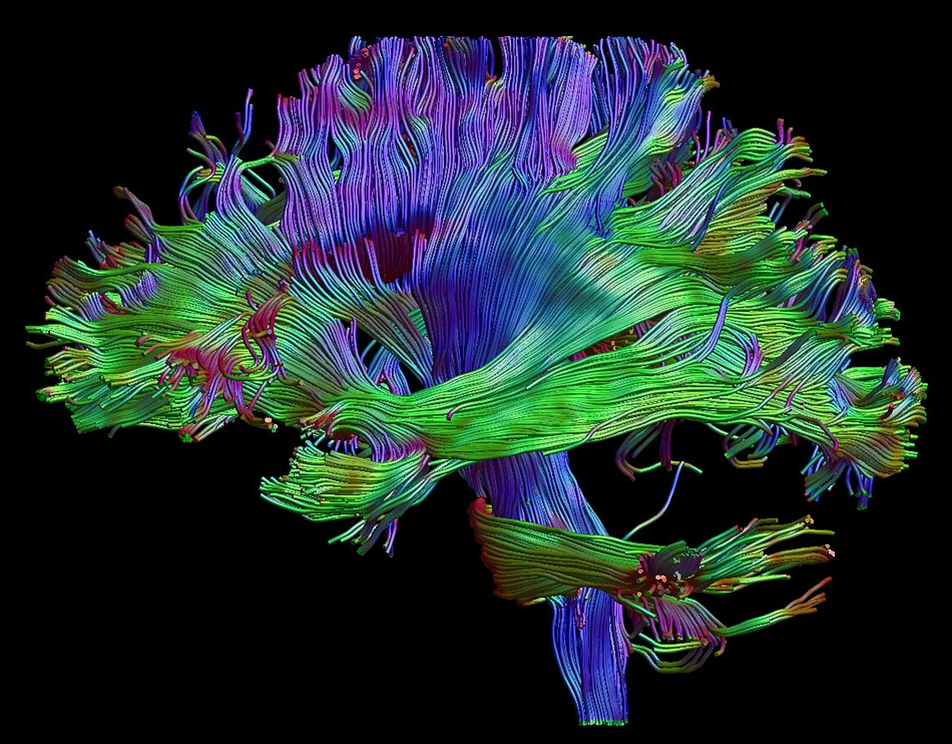
\includegraphics[width=.8\textwidth]{img/brain.png}
\end{center}
\end{frame}

\begin{frame}[t]{Evaluación}
\begin{center}
\includegraphics[width=\textwidth]{img/grppi-phardi.pdf}
\end{center}
\end{frame}

\begin{frame}[t]{Para saber más}
\begin{itemize}
  \item \textmark{C++ Concurrency in Action 2nd Edition}.
        Anthony Williams.
        Manning. 2019.

  \item \textmark{A Generic Parallel Pattern Interface for Stream and Data Processing}. 
        D. Rio, M. F. Dolz, J. Fernández, J. D. García. 
        Concurrency and Computation: Practice and Experience, 29(24): 12pp.
        2017.

  \item \textmark{Towards Automatic Parallelization of Stream Processing Applications}.
         M. F. Dolz, D. Rio, J. Fernández, J. D. García, J. Carretero. 
         IEEE Access. 6:39944–39961. 2018.
    
\end{itemize}
\end{frame}

\begin{frame}[t]{Resumen}
\begin{itemize}
  \item Uno de los lenguajes más usados en la industria del software.
  \vfill\pause
  \item Combinación única de:
    \begin{itemize}
      \item Capacidad para gestionar la complejidad.
      \item Espectacular rendimiento.
    \end{itemize}
  \vfill\pause
  \item Potencia de la programación genérica para trasladar cómputo 
        al tiempo de compilación.
  \vfill\pause
  \item Utilidades en la biblioteca: números complejos, generación de
        números aleatorios, funciones matemáticas especiales, álgebra lineal.
  \vfill\pause
  \item Fundamentos de nuevas características: contenedoros, iteradores, algoritmos,
        conceptos, contratos.
  \vfill\pause
  \item Paralelismo como ciudadano de primera clase. 
\end{itemize}
\end{frame}

\begin{frame}[t]{Recursos}
\begin{itemize}
  \item \textmark{ISO C++ Foundation}: \textgood{\url{https://isocpp.org/}}.
  \vfill
  \item \textmark{A Tour of C++, 2nd Edition}.
        Bjarne Stroustrup.
        Addison-Wesley.
        2018.
      
\end{itemize}
\end{frame}



\begin{frame}
\titlepage
\end{frame}

\end{document}
